\documentclass[a4paper]{article}
\usepackage{fontspec}\defaultfontfeatures{Ligatures=TeX}
% \usepackage{setspace}\setstretch{1.1} % \begin{spacing}{1.3}
\usepackage[a4paper,vmargin={2cm,3cm},hmargin={2cm,2cm}]{geometry}
%<--------------------------------------------------------------------------->%
\usepackage{settings}
%<--------------------------------------------------------------------------->%
%%% Title %%%
\title{How to compare the size of covariance matrices?}
\author{\href{https://jessekelighine.com}{jessekelighine.com}\\Jesse C.\ Chen\ 陳\,捷}
\date{\today}
%<--------------------------------------------------------------------------->%

\begin{document}

\maketitle

\begin{multicols}{2}

\noindent
Consider two covariance matrices $\AA_{n\times n}$ and $\BB_{n\times n}$.
We say that $\AA$ is \emph{larger} than $\BB$,
denoted by $\AA\geq \BB$ or $\AA\succsim \BB$,
if $\AA-\BB$ is semi-positive definite.
But why do we use matrix definiteness to compare the ``size'' of covariance matrices?

To understand this,
recall that a covariance matrix is not only symmetric,
but also positive semi-definite.
Let $\xx=(x_1,...,x_n)\T$ be a random vector.
Its covariance matrix is given by:
\begin{align*}
	\KK &\coloneqq \E{(\xx-\E{\xx})(\xx-\E{\xx})\T}.
\end{align*}
Now consider any constant vector $\vv\in\reals^n$.
We can examine the quadratic form:
\begin{align*}
	\vv\T \KK \vv &= \E(\vv\T(\xx-\E{\xx})(\vv\T(\xx-\E{\xx}))\T) \geq 0
\end{align*}
Therefore, the covariance matrix $\KK$ is always positive semi-definite.

There is another intuitive way of understanding the positive semi-definiteness.
Consider the same vector $\vv$ and the random vector $\xx$.
The dot product $\yy=\vv\T \xx$ is a projection of the random vector from $n$-dimensional
space on a one-dimensional space along the direction of $\vv$.
The variance of $\yy$ is given by
\begin{align*}
	\var(\yy)
	&= \E((\vv\T \xx)(\vv\T \xx)\T ) - \E(\vv\T \xx)\E(\vv\T \xx)\T  \\
	&= \vv\T \big(\E(\xx\xx\T ) - \E(\xx)\E(\xx)\T \big)\vv \\
	&= \vv\T \KK\vv.
\end{align*}
Notice that the variance of $\yy$ assumes the exact form as before.
Since variance is always non-negative, the covariance matrix must be positive semi-definite.
% Motivated by this intuition, we can now ask: how should we compare two covariance matrices?

With the two interpretations of covariance matrices in mind,
let's now compare the size of two covariance matrices.
Let $\xx=(x_1,...,x_n)\T$ and $\yy=(y_1,...,y_n)\T$ be random vectors, both with mean $(0,...,0)\T$ for simplicity.
Let $\AA=\E(\xx\xx\T)$ and $\BB=\E(\yy\yy\T)$ denote their respective covariance matrices.
Our goal is to compare $\AA$ and $\BB$ in some meaningful way.

A natural thought is to project both $\xx$ and $\yy$ onto an arbitrary direction $\vv\in\reals^n$,
then compare the variances of these one-dimensional projections.
Since each projection yields a non-negative scalar variance,
we can compare these scalar values across \emph{all} possible directions $\vv$.

Formally, consider any vector $\vv$,
consider the projection $\vv\T\xx$.
Its variance is
\begin{align*}
	\E((\vv\T \xx)^2)
	&= \E(\vv\T \xx\xx\T\vv) \\
	&= \vv\T\E(\xx\xx\T)\vv
	= \vv\T \AA\vv
\end{align*}
Similarly, for $\yy$ we have
\begin{align*}
	\E((\vv\T \yy)^2)
	= \vv\T \BB\vv.
\end{align*}
If for all $\vv$, we find:
\begin{align*}
	\vv\T \AA\vv - \vv\T \BB\vv
	= \vv\T (\AA - \BB)\vv
	\geq 0,
\end{align*}
then the matrix $\AA-\BB$, by definition, is positive semi-definite.
In this case, we say that $\AA$ is \emph{larger} than $\BB$ in the Loewner partial ordering. That is:
\begin{tcolorbox}[enhanced,sharp corners,frame hidden,boxrule=0sp,borderline west={3pt}{0pt}{black!70}]
	If $\AA-\BB$ is positive semi-definite,
	then \emph{for all possible directions $\vv$},
	the variance of the projection of $\xx$ exceeds or equals that of $\yy$.
	This defines the \href{https://en.wikipedia.org/wiki/Loewner_order}{Loewner ordering}.
\end{tcolorbox}

This interpretation is intuitive when visualized geometrically.
Imagine two random vectors $\xx$ and $\yy$ in $\reals^2$, whose distributions are represented by ellipses:
\begin{center}
	\includegraphics[width=0.2\textwidth]{figures/visual-1.pdf}
	\hspace{0.5em}
	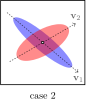
\includegraphics[width=0.2\textwidth]{figures/visual-2.pdf}
\end{center}
Let the blue ellipse represent the distribution $\xx$ with covariance matrix $\AA$,
and let the red ellipse represent the distribution $\yy$ with covariance matrix $\BB$.

In case 1, $\AA$ is \emph{larger} than $\BB$
since the blue ellipse fully encloses the red one,
indicating that in \emph{every direction}, the variance of $\xx$ exceeds that of $\yy$.
However, the same statement is not true in case 2.
In some directions, e.g.\ along $\vv_1$, the variance of $\xx$ is larger;
in other directions, e.g.\ along $\vv_2$, the variance of $\yy$ is larger.
Thus, $\AA$ and $\BB$ are not comparable by Loewner ordering,
meaning that it does not make sense to say that one covariance matrix is larger than the other.
\asDemonstrated

\end{multicols}

\end{document}
